
\documentclass[xcolor=dvipsnames]{beamer} % dvipsnames gives more built-in colors
\usepackage[utf8]{inputenc}
\usepackage[spanish]{babel}

\mode<presentation> {

\usetheme{CambridgeUS}

%\setbeamertemplate{footline} % To remove the footer line in all slides uncomment this line
\setbeamertemplate{footline}[page number] % To replace the footer line in all slides with a simple slide count uncomment this line

\setbeamertemplate{navigation symbols}{} % To remove the navigation symbols from

\definecolor{utfsmred}{HTML}{D60019}
\definecolor{utfsmyellow}{HTML}{F7AE00}
\definecolor{utfsmgreen}{HTML}{008452}
\definecolor{utfsmblue}{HTML}{004B85}


\newenvironment<>{rosa}[1][]{
  \setbeamercolor{block title example}{fg=white,bg=blue!75!black}%
  \begin{example}#2[#1]}{
  \end{example}
}



\usecolortheme[named=utfsmblue]{structure}
\setbeamercolor{titlelike}{parent=structure,fg=utfsmblue}
\setbeamercolor{frametitle}{fg=utfsmblue}

%\setbeamercolor{section in head/foot}{bg=Brown}
%\setbeamercolor{author in head/foot}{bg=Brown}
%\setbeamercolor{date in head/foot}{fg=Brown}

\setbeamercolor*{enumerate item}{fg=utfsmred}
\setbeamercolor*{enumerate subitem}{fg=utfsmred}
\setbeamercolor*{enumerate subsubitem}{fg=utfsmred}

\setbeamercolor*{itemize item}{fg=utfsmred}
\setbeamercolor*{itemize subitem}{fg=utfsmred}
\setbeamercolor*{itemize subsubitem}{fg=utfsmred}

\setbeamercolor{item projected}{bg=utfsmred}


\setbeamertemplate{itemize items}[square]
\setbeamertemplate{enumerate items}[default]


\setbeamercolor{section in head/foot}{bg=utfsmblue}

\setbeamercolor{block title}{bg=utfsmblue!80,fg=white}
\setbeamercolor{block title alerted}{bg=utfsmred!80,fg=white}
\setbeamercolor{block title example}{bg=utfsmgreen!80,fg=white}

\setbeamertemplate{sections/subsections in toc}[square]
\setbeamercolor{section number projected}{bg=utfsmblue,fg=white}


}


\usepackage{graphicx} % Allows including images
\usepackage{booktabs} % Allows the use of \toprule, \midrule and \bottomrule in tables
\usepackage{listings}
\lstset{ %
language=C,
basicstyle=\normalsize\ttfamily,
keywordstyle=,
numbers=none,
numberstyle=\tiny\ttfamily,
stepnumber=1,
showspaces=false,
showstringspaces=false,
showtabs=false,
breaklines=true,
frame=tb,
framerule=0.5pt,
tabsize=4,
framexleftmargin=0.5em,
framexrightmargin=0.5em,
xleftmargin=0.5em,
xrightmargin=0.5em,
}

%----------------------------------------------------------------------------------------
%	TITLE PAGE
%----------------------------------------------------------------------------------------

\title{File System Hierarchy Standard (FHS)}
\subtitle{\small{Seminario de Desarrollo de Software - Casa Central.}}
\author{Maximiliano Osorio\\\small{mosorio@inf.utfsm.cl}} 
\institute[UTFSM]
{
Universidad Técnica Federico Santa María
\medskip
}
\date{\today} % Date, can be changed to a custom date

\begin{document}

\maketitle


\begin{frame}{FHS}
	\begin{figure}
		\centering
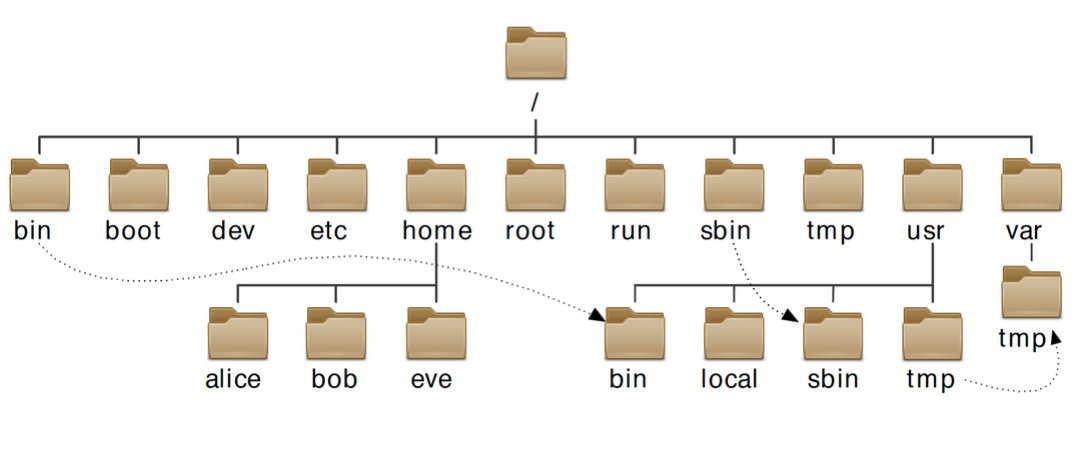
\includegraphics[width=\textwidth,height=0.8\textheight,keepaspectratio]{images/fhs}	\end{figure}
\end{frame}


\begin{frame}[fragile]
\frametitle{FHS}

\begin{itemize}[<+->]
	\item \textbf{/boot/}: Contiene los archivos estaticos necesarios para el booteo del sistema. e.g. kernel.
	\item \textbf{/usr/bin/:} Binario del sistema, tiene un enlace \textbf{/bin/}
	\item \textbf{/dev}: Contiene los dispositivos en el sistema.
	\item \textbf{/etc/}: Es reservado para los archivos de configuración que son locales en la maquina. No debe contener binarios.
	\item \textbf{/media/}: Debe contener los puntos de montajes como USB...
	\item \textbf{/mnt/}: Reservado para puntos de montaje temporales.
	\item \textbf{/opt/}: Es normalmente reservado para software y addons y que no son parte de la instalación yum.

	\end{itemize}
\end{frame}


\begin{frame}[fragile]
\frametitle{FHS}

\begin{itemize}[<+->]

	\item \textbf{/proc/}: Contiene principalmente archivos de texto, sistema de archivos virtuales que documentan al núcleo y el estado de los procesos en archivos de texto (por ejemplo, uptime, network.
	\item \textbf{/srv/}: Lugar específico de datos que son servidos por el sistema.
	\item \textbf{/var/}: Archivos variables, tales como logs, archivos spool, bases de datos, archivos de e-mail temporales, y algunos archivos temporales en general. Generalmente actúa como un registro del sistema. Ayuda a encontrar los orígenes de un problema.
	\item \textbf{/run}: es un directorio como un filesystem temporal que guarda información volátil.
	\end{itemize}
\end{frame}




\begin{frame}{FHS}
	\begin{figure}
		\centering
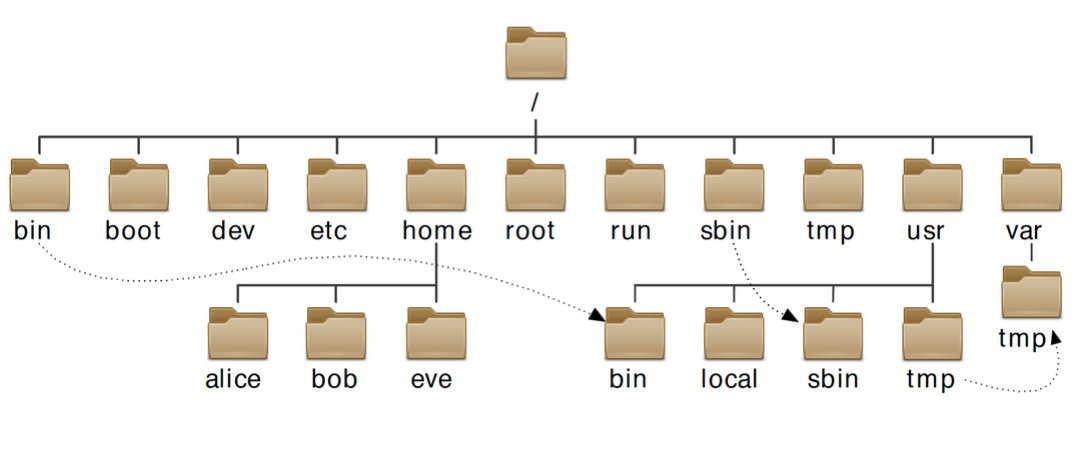
\includegraphics[width=\textwidth,height=0.8\textheight,keepaspectratio]{images/fhs}	\end{figure}
\end{frame}

\begin{frame}[fragile]
\frametitle{Rutas}

\begin{itemize}
\item Absolutas: Comienzan con /.  (e.g. /root/, /usr/share/)
\item Relativas: Relativas a donde se encuentran, (e.g log/messages es relativa a /var)
\end{itemize}
\begin{block}{Consejo}
	Las rutas con espacio son aceptadas en los archivos, pero un espacio es un delimitador de la shell. Por lo tanto es bueno evitar el uso del espacio para nombres de archivos y directorios.
\end{block}
\end{frame}

\begin{frame}[fragile]
\frametitle{Navegando: cd}
\begin{itemize}
	\item \textbf{cd \~} mueve al directorio home del usuario.\end{itemize}
\begin{lstlisting}
[mosorio@ssh ~]$ cd /usr/share/
[mosorio@ssh share]$ pwd
/usr/share
[mosorio@ssh share]$ cd ~
[mosorio@ssh ~]$ pwd
/home/mosorio
\end{lstlisting}
\end{frame}


\begin{frame}[fragile]
\frametitle{Navegando: cd, pwd}
\begin{itemize}
	\item \textbf{pwd} muestra la ruta absoluta. 

\end{itemize}
\begin{lstlisting}
[mosorio@ssh public_html]$ pwd
/home/mosorio/public_html
[mosorio@ssh ~]$ cd ~
[mosorio@ssh ~]$ pwd
/home/mosorio
\end{lstlisting}
\end{frame}


\begin{frame}[fragile]
\frametitle{Navegando: cd, pwd}
\begin{itemize}
	\item \textbf{pwd} muestra la ruta absoluta. 
	\item \textbf{cd ..} mueve al directorio que está un nivel arriba
\end{itemize}
\begin{lstlisting}
[root@losvilos usr]# pwd
/usr
[root@losvilos usr]# ls
bin  games  include  lib  lib64  libexec  local  locale  sbin  share  src  tmp
[root@losvilos usr]# cd lib/gems/
[root@losvilos gems]# pwd
/usr/lib/gems
[root@losvilos gems]# cd ..
[root@losvilos lib]# pwd
/usr/lib
[root@losvilos lib]# cd
[root@losvilos ~]# pwd
/root
\end{lstlisting}
\end{frame}


\begin{frame}[fragile]
\frametitle{Navegando: cd}
\begin{itemize}
	\item \textbf{cd \-} mueve al directorio usado anteriormente.
\end{itemize}
\begin{lstlisting}
[mosorio@ssh ~]$ cd /usr/share/
[mosorio@ssh share]$ pwd
/usr/share
[mosorio@ssh share]$ cd ~
[mosorio@ssh ~]$ pwd
/home/mosorio
[mosorio@ssh ~]$ cd -
/usr/share
\end{lstlisting}
\end{frame}



\begin{frame}[fragile]
\frametitle{Navegando: touch}
\begin{itemize}
	\item \textbf{touch} crea un archivo vacío.\end{itemize}
\begin{lstlisting}
[root@losvilos curso]# touch never
[root@losvilos curso]# touch gonna
[root@losvilos curso]# touch give
[root@losvilos curso]# touch you
[root@losvilos curso]# touch up

[root@losvilos curso]# ls
give  gonna  never  up  you
\end{lstlisting}
\end{frame}




\begin{frame}[fragile]
\frametitle{Navegando: ls}
\begin{lstlisting}[basicstyle=\small]
[root@losvilos curso]# ls -la
total 0
drwxr-xr-x.  2 root root  160 Oct  7 15:09 .
drwxrwxrwt. 46 root root 8860 Oct  7 15:08 ..
-rw-r--r--.  1 root root    0 Oct  7 15:09 .astley
-rw-r--r--.  1 root root    0 Oct  7 15:08 give
-rw-r--r--.  1 root root    0 Oct  7 15:08 gonna
-rw-r--r--.  1 root root    0 Oct  7 15:08 never
-rw-r--r--.  1 root root    0 Oct  7 15:08 up
-rw-r--r--.  1 root root    0 Oct  7 15:08 you
\end{lstlisting}
\end{frame}

\begin{frame}[fragile]
\frametitle{Navegando: ls}
\begin{lstlisting}[basicstyle=\small]
ls -lR
total 0
drwxr-xr-x  5 mosorio  staff  170 Oct  7 15:17 a
drwxr-xr-x  3 mosorio  staff  102 Oct  7 15:17 b
drwxr-xr-x  3 mosorio  staff  102 Oct  7 15:17 c

./a:
total 0
-rw-r--r--  1 mosorio  staff  0 Oct  7 15:17 a1
-rw-r--r--  1 mosorio  staff  0 Oct  7 15:17 a2
-rw-r--r--  1 mosorio  staff  0 Oct  7 15:17 a3

./b:
total 0
-rw-r--r--  1 mosorio  staff  0 Oct  7 15:17 b3

\end{lstlisting}

\end{frame}

\begin{frame}[fragile]
\frametitle{}
\begin{figure}
\centering
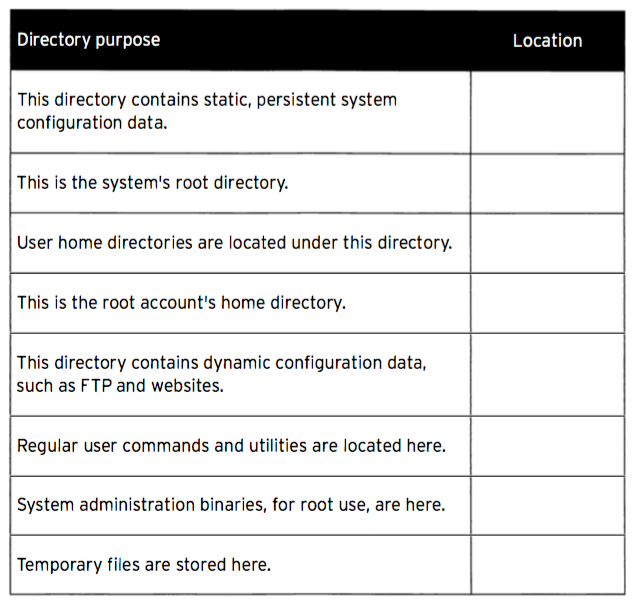
\includegraphics[width=\textwidth,height=1\textheight,keepaspectratio]{images/q1}
\end{figure}
\end{frame}
%------------------------------------------------

\begin{frame}[fragile]
\frametitle{}
\begin{figure}
\centering
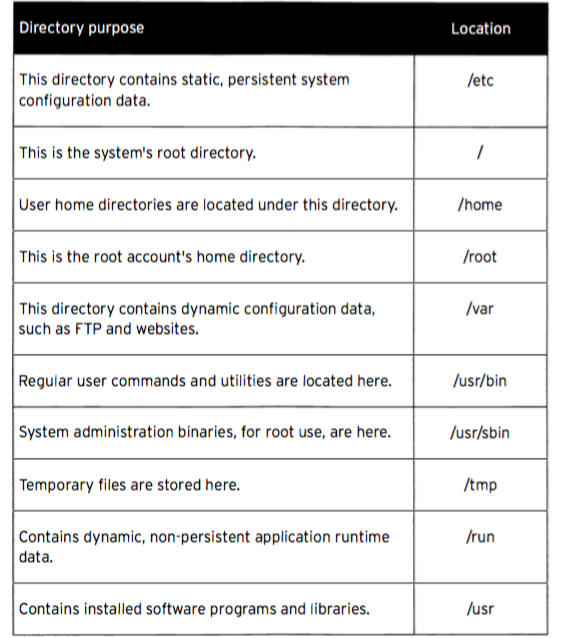
\includegraphics[width=\textwidth,height=1\textheight,keepaspectratio]{images/r1}
\end{figure}
\end{frame}
%------------------------------------------------
\begin{frame}[fragile]
\frametitle{}
\begin{figure}
\centering
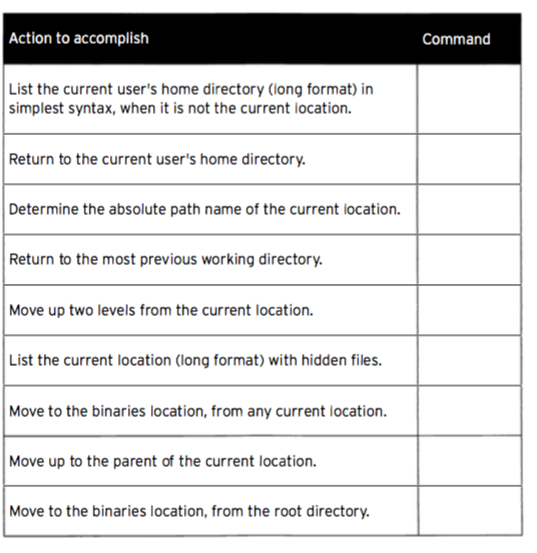
\includegraphics[width=\textwidth,height=1\textheight,keepaspectratio]{images/q2}
\end{figure}
\end{frame}
%------------------------------------------------
\begin{frame}[fragile]
\frametitle{}
\begin{figure}
\centering
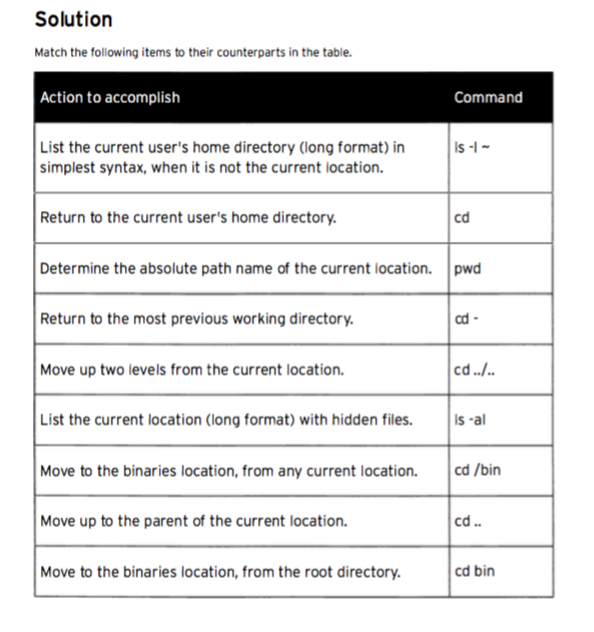
\includegraphics[width=\textwidth,height=1\textheight,keepaspectratio]{images/r2}
\end{figure}
\end{frame}
%------------------------------------------------






\end{document}